\subsubsection{9$^{\circ}$ Incremento}
		\subsubsubsection{Prospetto orario}
		Durante il 9$^{\circ}$ incremento la distribuzione oraria preventivata dei ruoli di ogni componente del gruppo sarà la seguente:
		\rowcolors{2}{lightRowColor}{darkRowColor}
		\begin{longtable}{
				>{\centering}p{0.25\textwidth}
				>{\centering}p{0.05\textwidth}
				>{\centering}p{0.05\textwidth}
				>{\centering}p{0.05\textwidth}
				>{\centering}p{0.05\textwidth}
				>{\centering}p{0.05\textwidth}
				>{\centering}p{0.05\textwidth}
				>{\centering\arraybackslash}p{0.15\textwidth} }
			
			\coloredTableHead
			\textbf{\color{white}Nome} &
			\textbf{\color{white}Rp} &
			\textbf{\color{white}As} &
			\textbf{\color{white}An} &
			\textbf{\color{white}Pt} &
			\textbf{\color{white}Pr} &
			\textbf{\color{white}Vf} &
			\textbf{\color{white}Totale}
			\tabularnewline
			\endhead
			
			% Contenuto della tabella
			%    Rp & As & An & Pt & Pr & Vf & Totale \\
			\VB & - & 2  & - & - & - & 4 & 6 \\
			\LB & - & -  & - & 4 & - & - & 4 \\
			\NF & - & 4  & - & - & - & - & 4 \\
			\EG & 2 & -  & - & 2 & - & - & 4 \\
			\FJ & - & -  & - & - & - & 4 & 4 \\
			\MP & - & -  & - & 2 & - & 3 & 5 \\
			\AS & - & -  & - & 2 & - & 2 & 4 \\
			\AZ & - & 2  & - & - & - & 2 & 4 \\
			\textbf{Ore totali per ruolo} & 2 & 8 & 0 & 10 & 0 & 15 & 35 \\
			
			\rowcolor{white}\caption {Suddivisione oraria del 9$^{\circ}$ incremento} \\
			
		\end{longtable}
		
		% Grafico
		\begin{figure}[H]
			\centering
			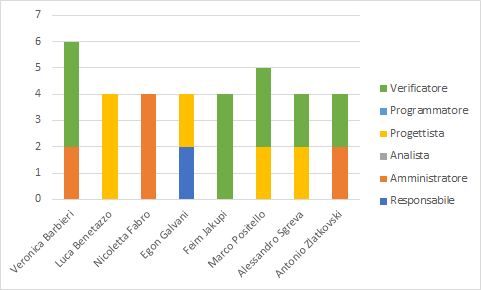
\includegraphics[width=0.7\textwidth]{./res/img/preventivi/inc9_po.png}
			\caption{Suddivisione oraria del 9$^{\circ}$ incremento}
		\end{figure}
	
		\subsubsubsection{Prospetto economico}
		In base al prospetto orario, quello economico sarà il seguente: 
		\rowcolors{2}{lightRowColor}{darkRowColor}
		\begin{longtable}{
				>{\centering}p{0.25\textwidth}
				>{\centering}p{0.05\textwidth}
				>{\centering\arraybackslash}p{0.15\textwidth} }
			
			\coloredTableHead
			\textbf{\color{white}Ruolo} &
			\textbf{\color{white}Ore} &
			\textbf{\color{white}Costo in \euro{}}
			\tabularnewline
			\endhead
			
			% Contenuto della tabella
			% Ruolo & Ore & Costo \\
			Responsabile    & 2  & 60,00 \\
			Amministratore  & 8  & 160,00 \\
			Analista        & 0  & 0,00 \\
			Progettista     & 10  & 220,00 \\
			Programmatore   & 0  & 0,00 \\
			Verificatore    & 15  & 225,00 \\
			\textbf{Totale} & 35 & 665,00 \\
			
			\rowcolor{white}\caption {Prospetto dei costi per il 9$^{\circ}$ incremento}	\\
			
		\end{longtable}
		
		% Grafico
		Rappresentazione grafica della distribuzione dei ruoli:
		\begin{figure}[H]
			\centering
			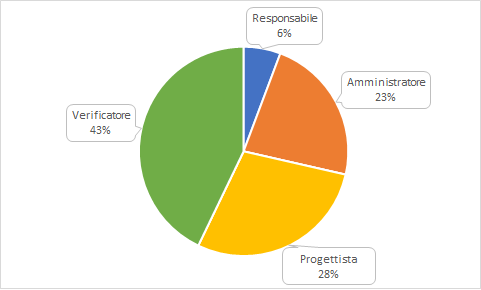
\includegraphics[width=0.7\textwidth]{./res/img/preventivi/inc9_pe.png}
			\caption{Prospetto economico del 9$^{\circ}$ incremento}
		\end{figure}